\section{Measurements of radiation damage on sensors}
\label{sec:measurements}
{\it Editors: A. De Cosa, B. Nachman, P. Collins}  \\
{\it Contibuting authors: J.~Agram, A. De Cosa, B.~Nachman, W.~Barter, J.~Beyer, M.~Baselga, F.~Feindt, A.~Grummer, J.~Hunt, T.~Kondo, V.~Lima, K.~Mochizuki, J.~Sonneveld, M.~Vignali}  \\

\noindent 
General introduction on the effects of radiation on sensors, though I propose details should go in section~\ref{sec:effects}. Here we should focus on the experiment measurements, and how they compare to the predictions from simulation and modelling. \\
For presenting results I think easiest to summarise studies and conclusions for each experiment first, as we did in the workshops, then try to extract combined conclusions? A crude outline given below ...

\subsection{Measurements}

Several measurements from ATLAS pixels can be found in Ref.~\cite{Aaboud:2019wgd}, from the LHCb tracker~\cite{AbellanBeteta:2018wif}, LHCb VELO~\cite{Akiba:2633496}, ...

\subsubsection{Leakage Current}

Fig.~\ref{lab:sensormeasurements:Leakage:ATLAS1}.

\begin{figure}[h!]
\centering
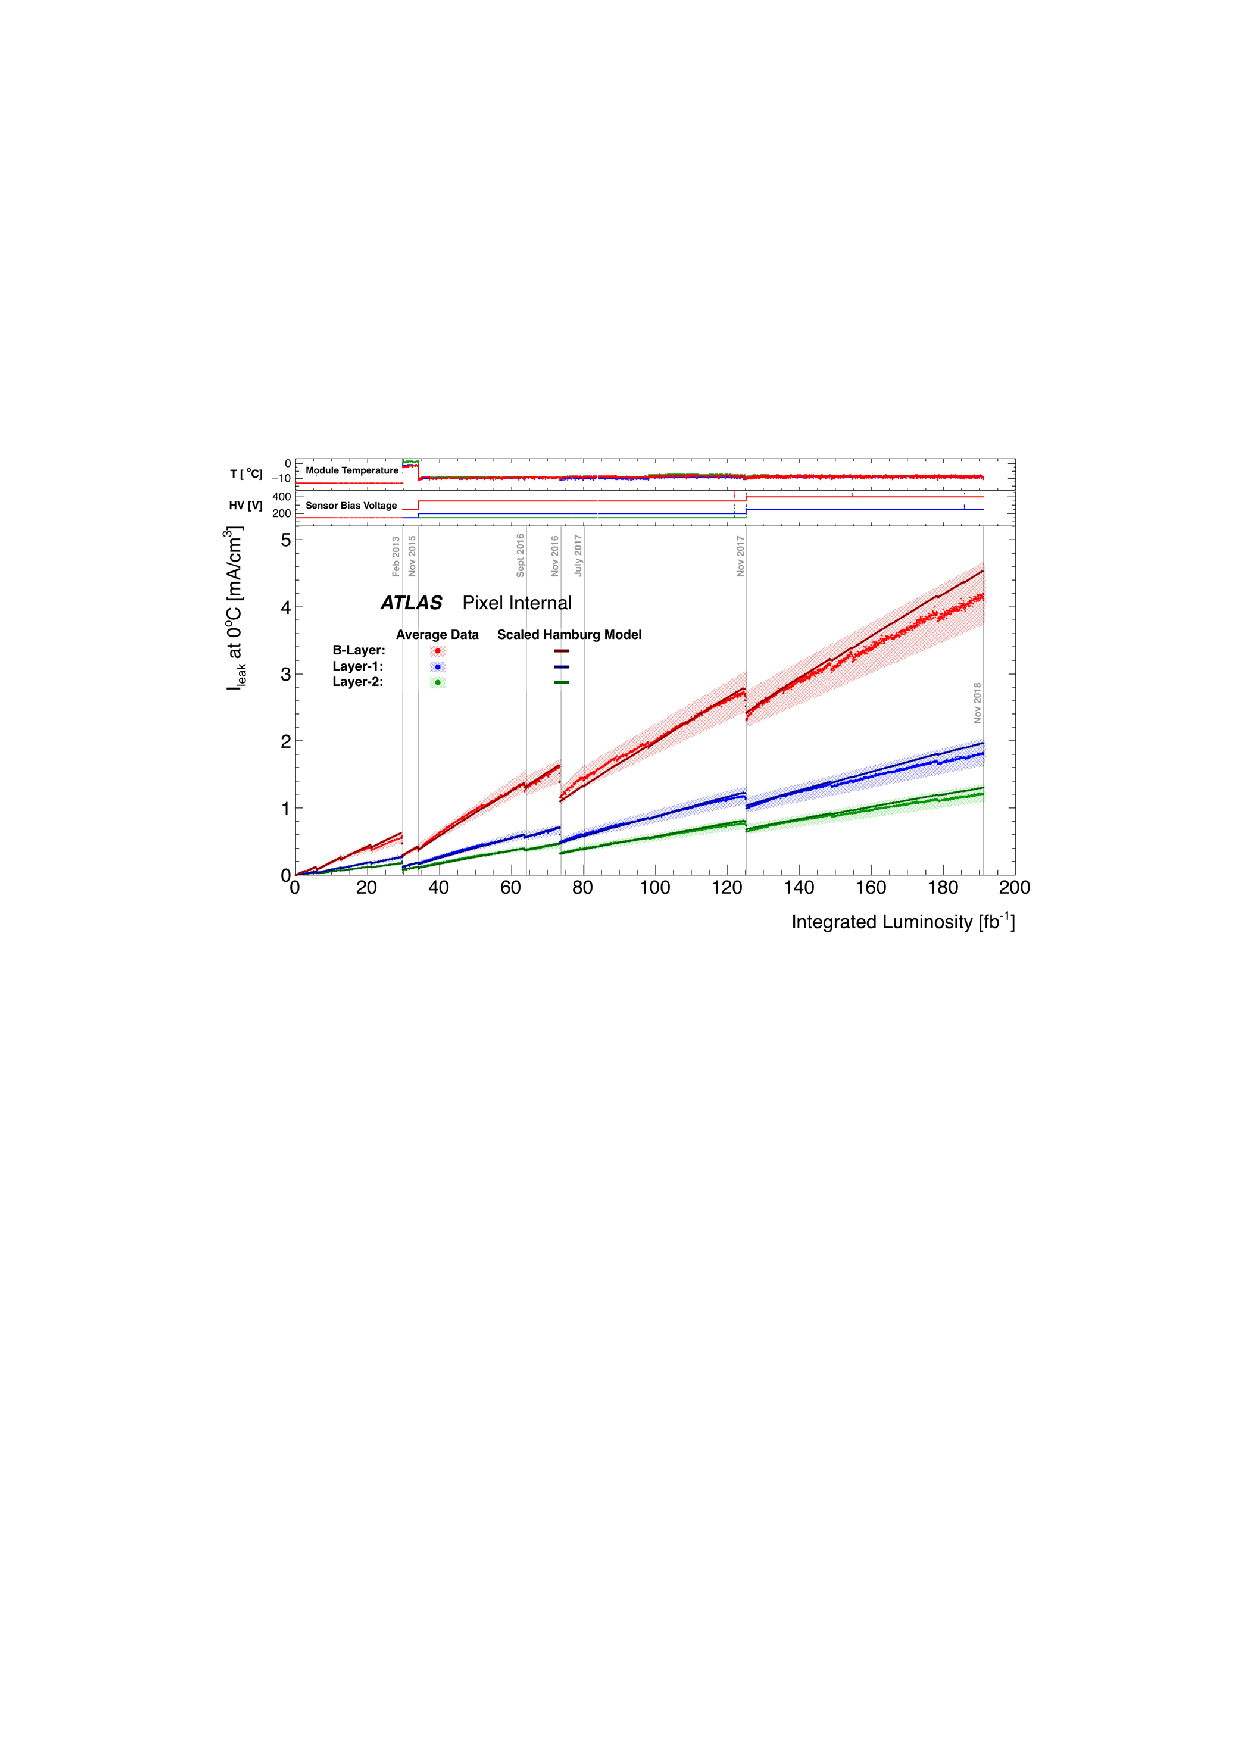
\includegraphics[width=0.52\textwidth]{figures/SensorMeasurements/LeakageCurrent/ATLAS-blayerL1L2}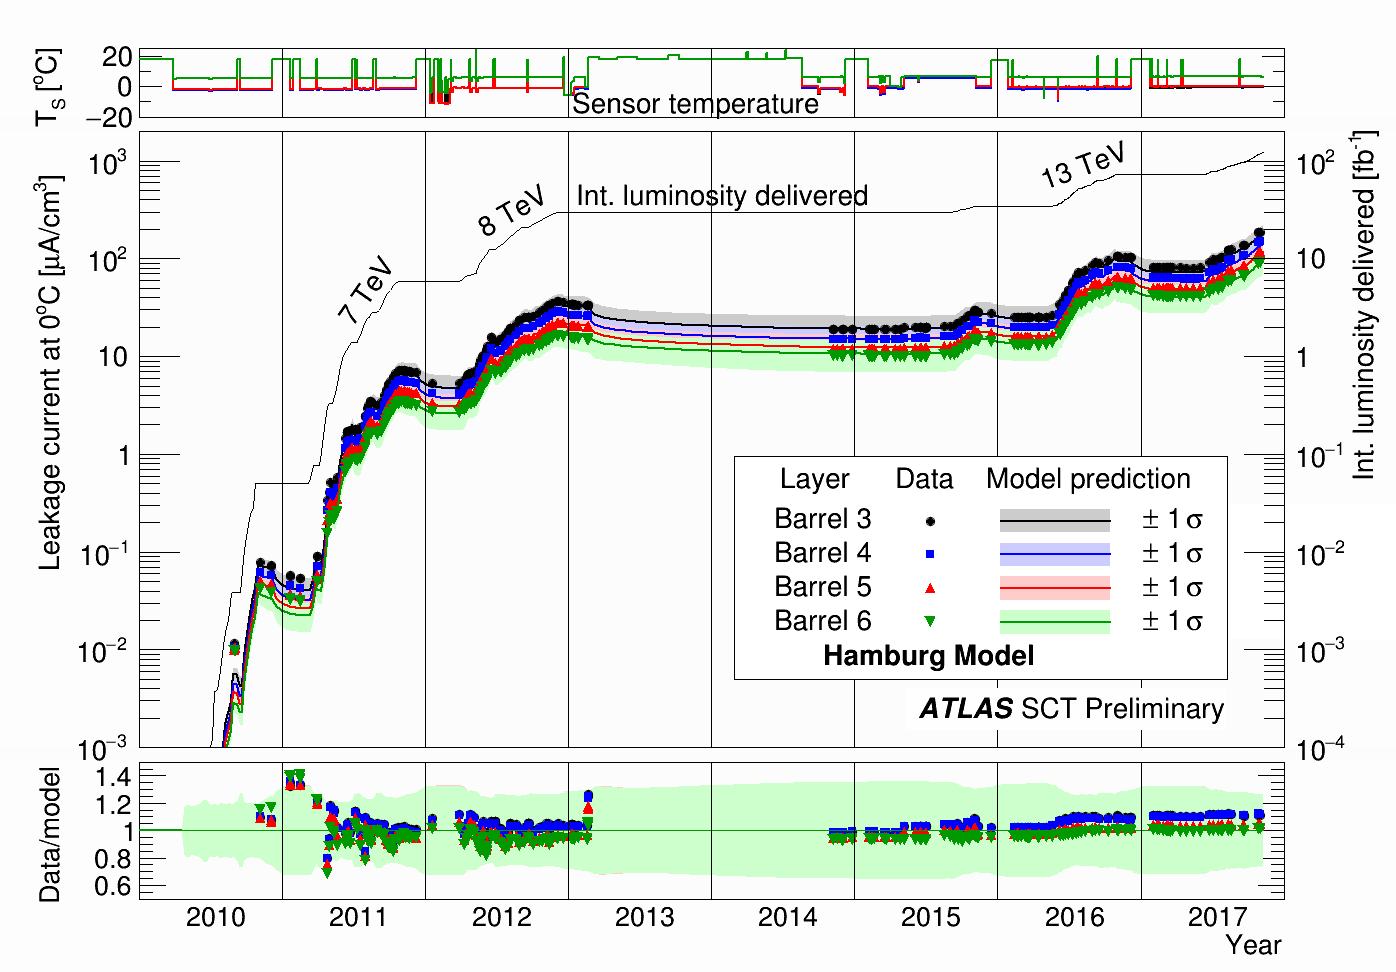
\includegraphics[width=0.45\textwidth]{figures/SensorMeasurements/LeakageCurrent/ATLAS-SCT.png}
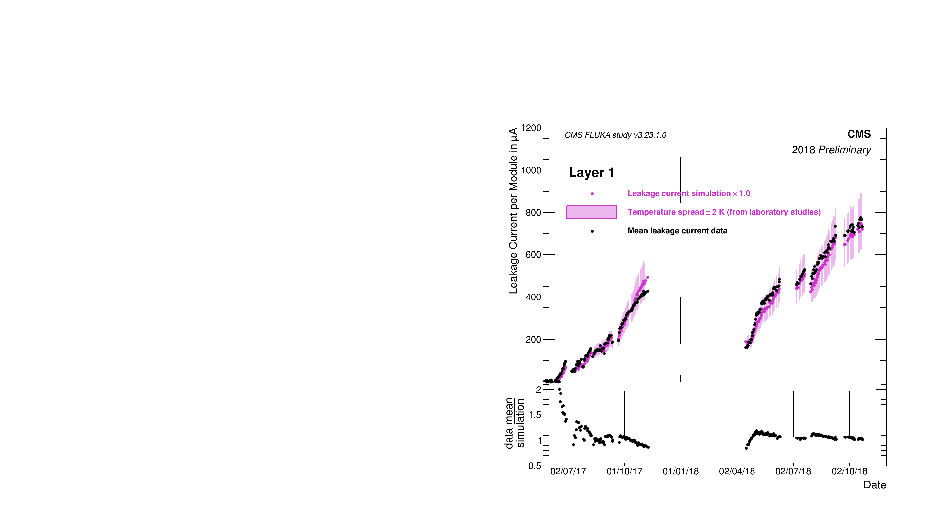
\includegraphics[width=0.4\textwidth]{figures/SensorMeasurements/LeakageCurrent/CMS-pixels}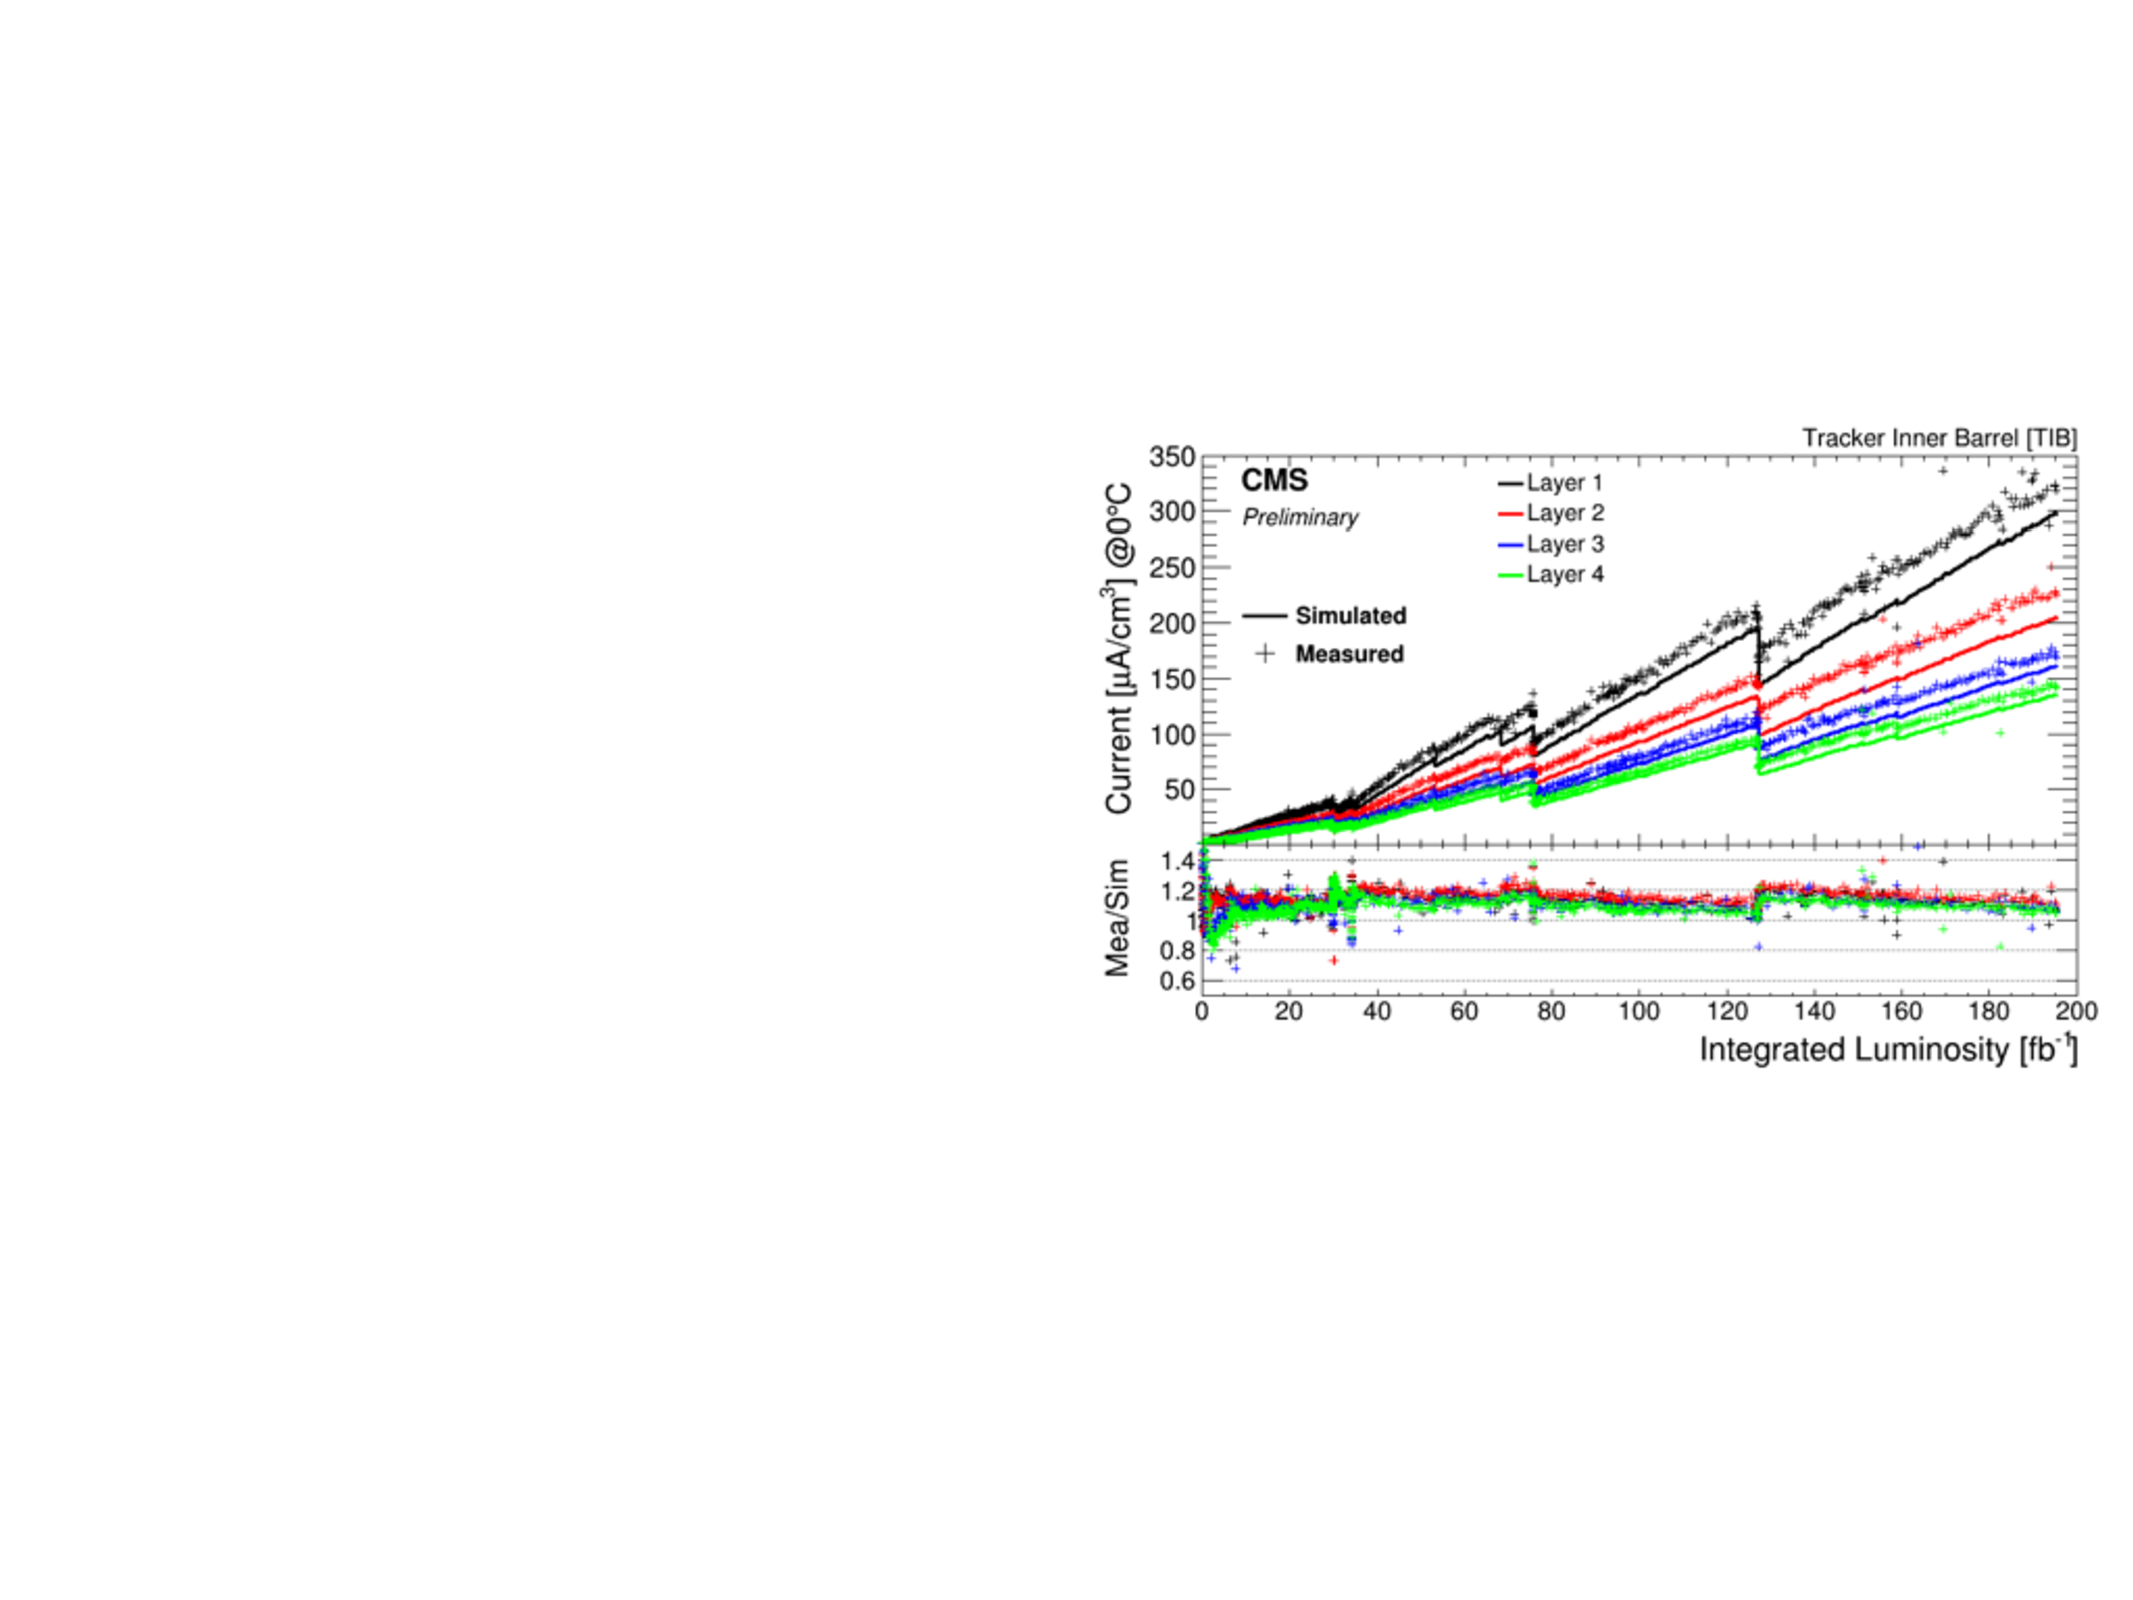
\includegraphics[width=0.55\textwidth]{figures/SensorMeasurements/LeakageCurrent/CMS-strips}
\caption{Top left: ATLAS leakage current from the outer three pixel layers, from Ref.~\cite{ATL-INDET-PUB-2019-001}.  The IBL leakage current measurement can be found in Ref.~\cite{ATL-INDET-INT-2019-012}.  Top right: ATLAS SCT, from Ref.~\cite{ATL-SCT-2018-002}.  Bottom left: CMS pixels.  Bottom right: CMS strips.}
\label{lab:sensormeasurements:Leakage:ATLAS1}
\end{figure}

\subsubsection{Depletion Voltage}

Fig.~\ref{lab:sensormeasurements:Depletion:ATLAS1}.

\begin{figure}[h!]
\centering
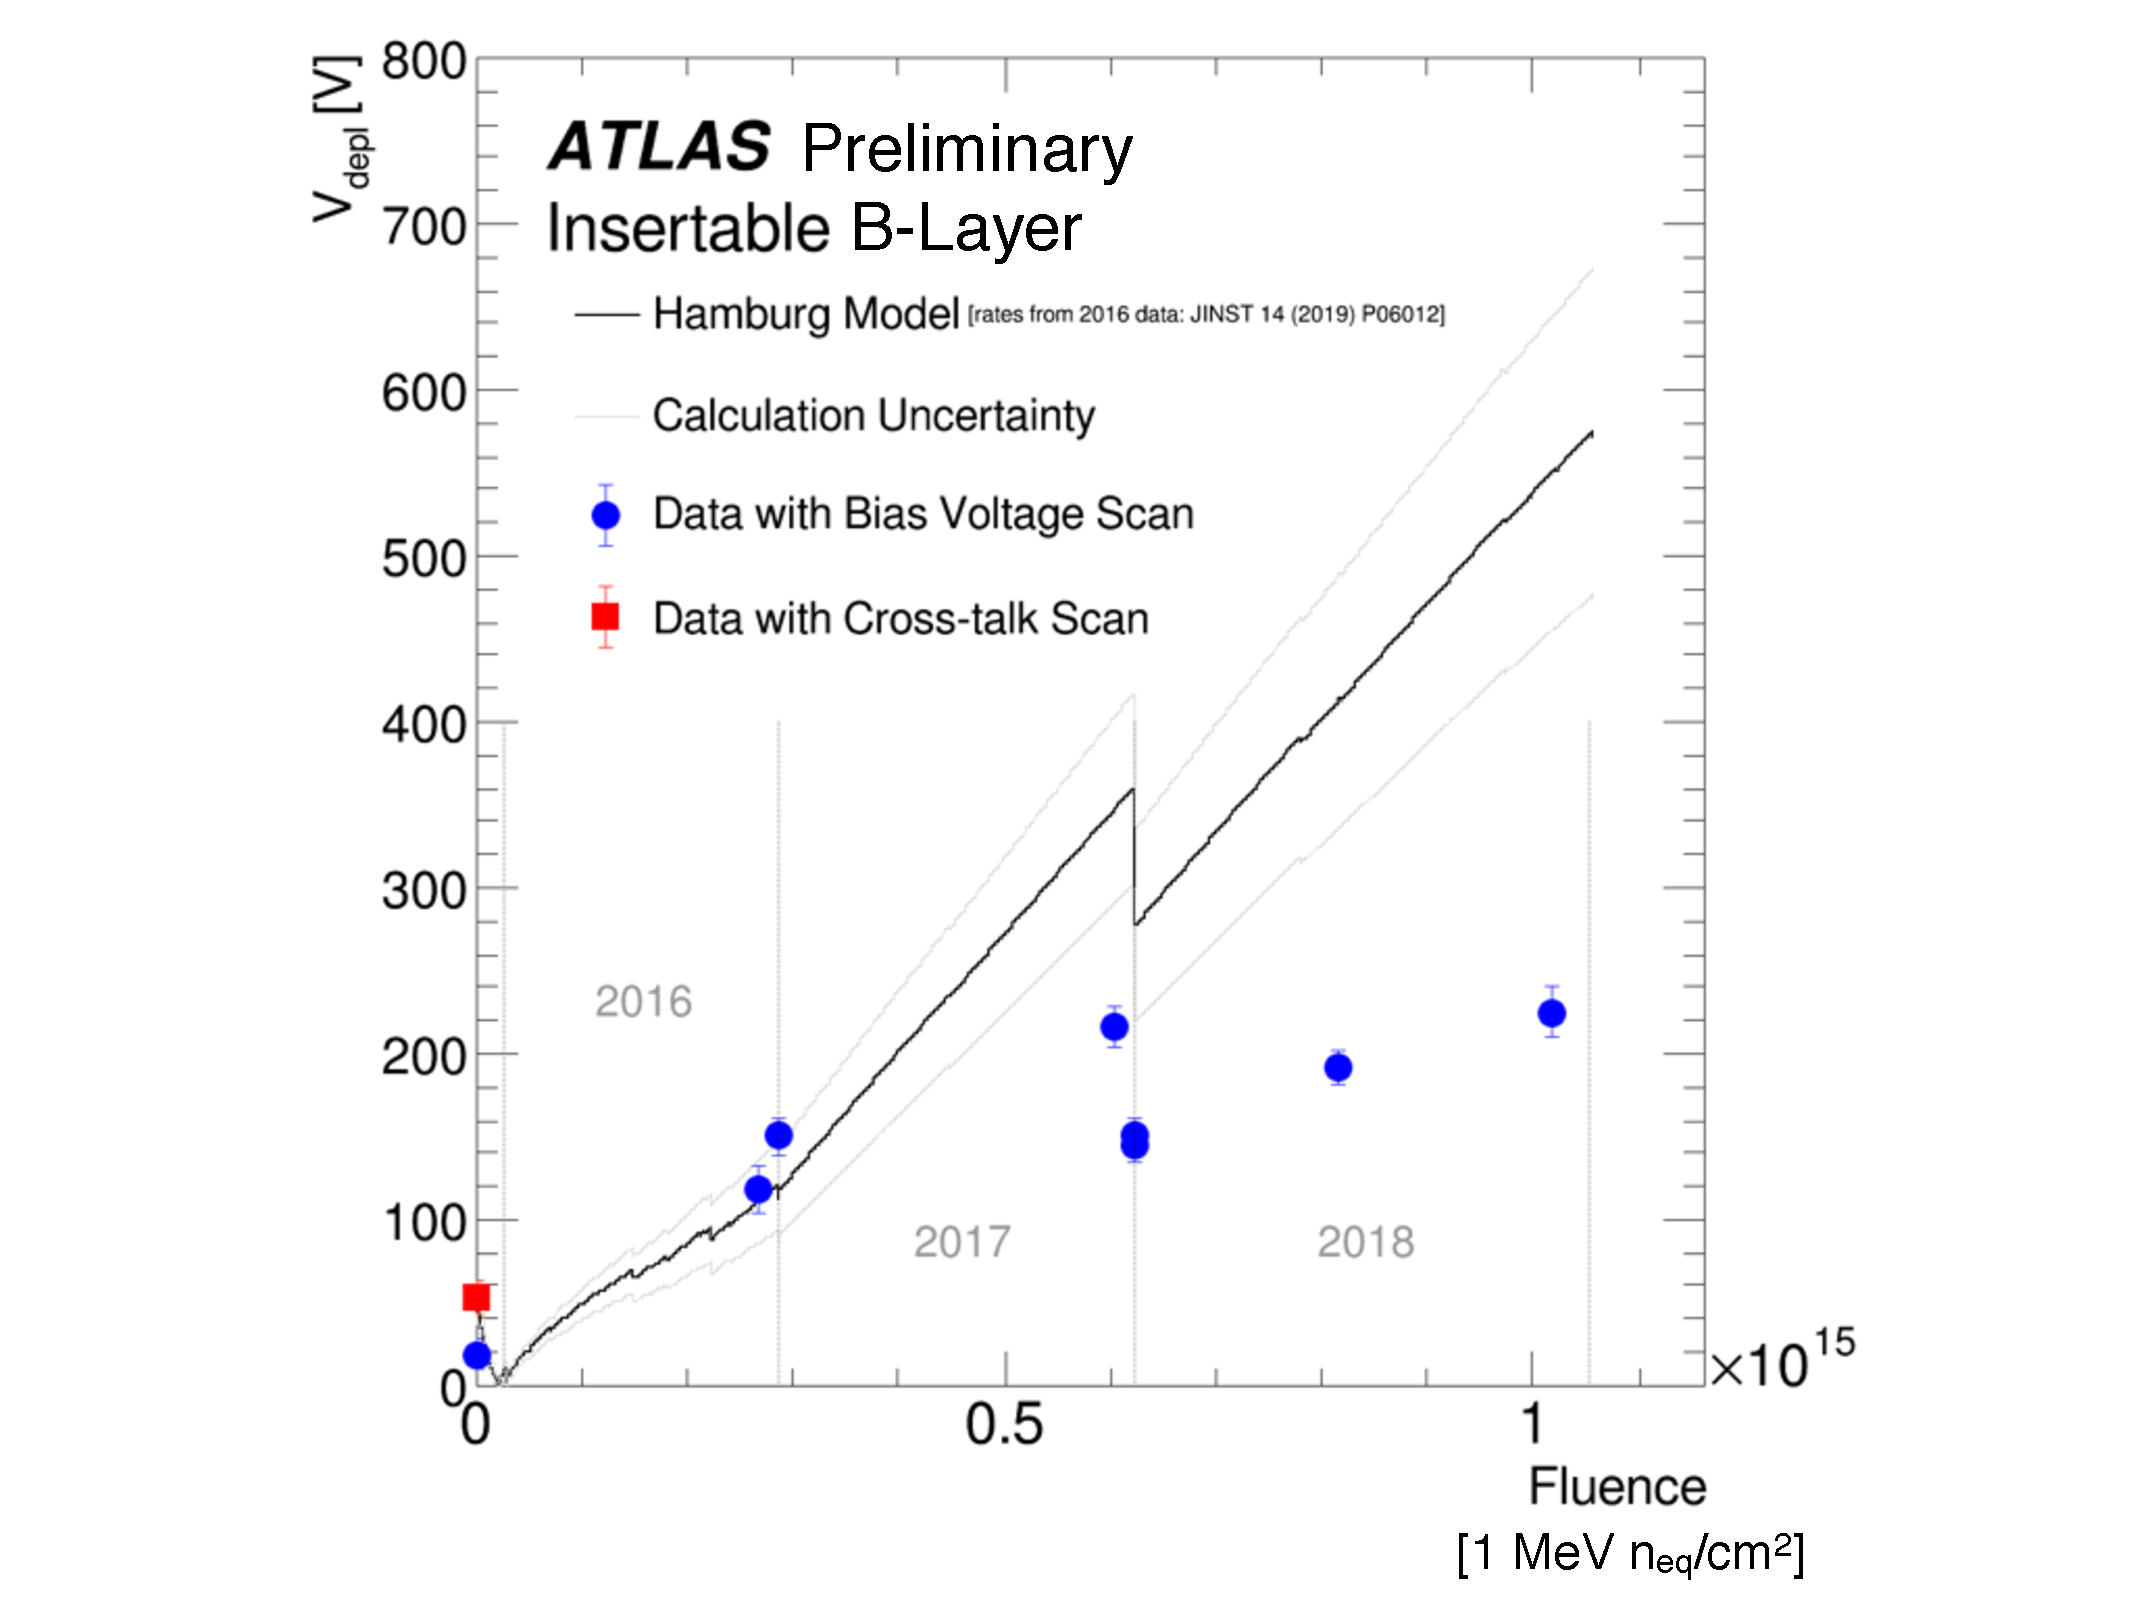
\includegraphics[width=0.55\textwidth]{figures/SensorMeasurements/DepletionVoltage/atlas-ibl-depletion.pdf}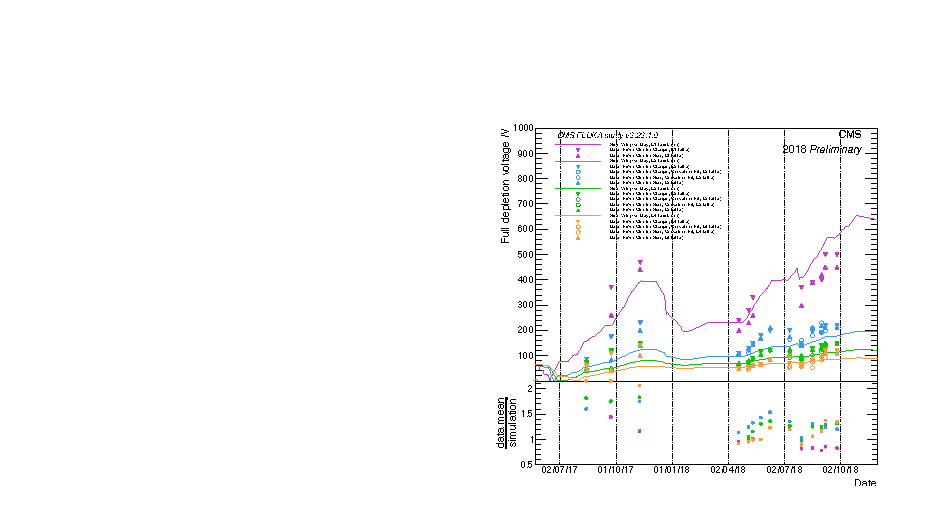
\includegraphics[width=0.45\textwidth]{figures/SensorMeasurements/DepletionVoltage/cms-pixels}\\
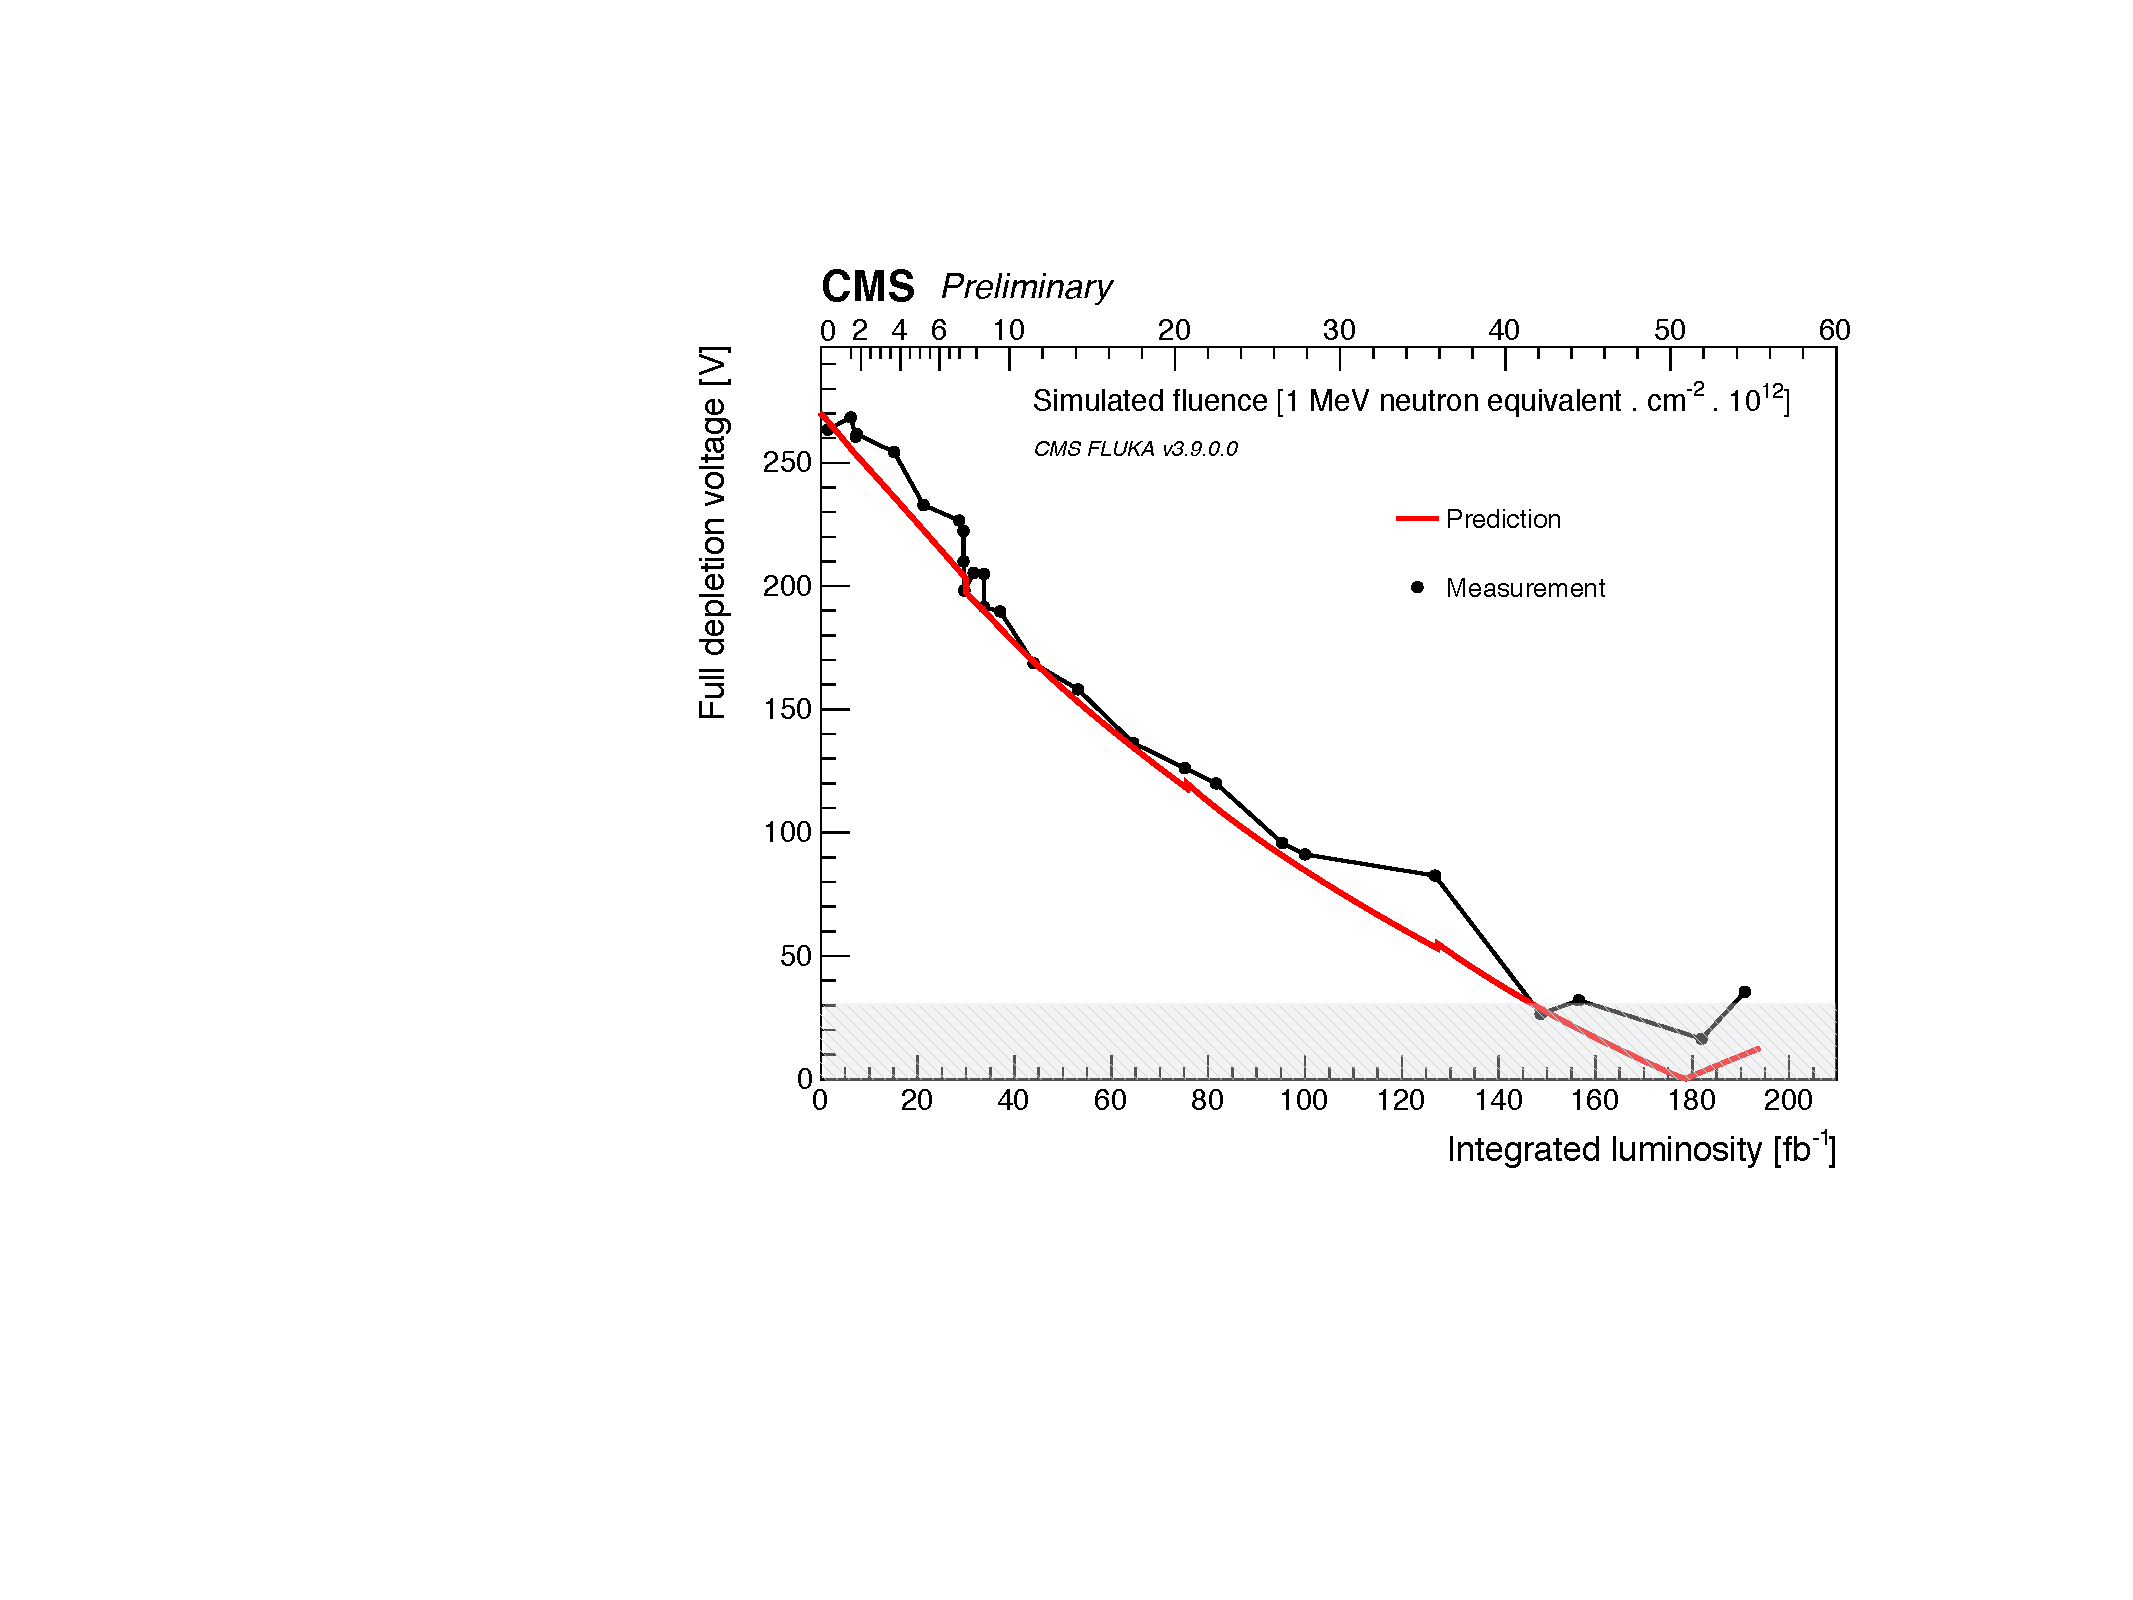
\includegraphics[width=0.47\textwidth]{figures/SensorMeasurements/DepletionVoltage/cms-strips}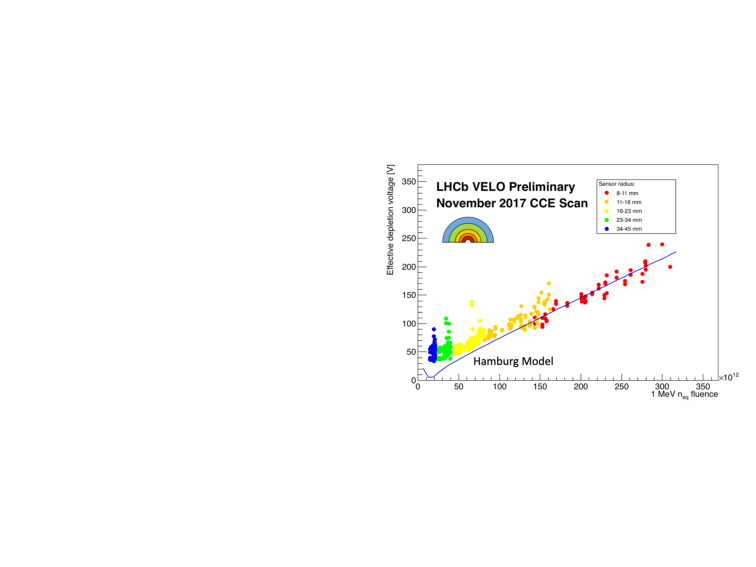
\includegraphics[width=0.53\textwidth]{figures/SensorMeasurements/DepletionVoltage/lhcb-velo}
\caption{Top left: ATLAS IBL, figure from Ref.~\cite{ATL-INDET-INT-2019-016}.  Top right: CMS pixels.  Bottom left: CMS strips.  Bottom right: LHCb VELO.}
\label{lab:sensormeasurements:Depletion:ATLAS1}
\end{figure}

\subsubsection{Charge Collection, Hit Efficiency, and Cluster Size}

Fig.~\ref{lab:sensormeasurements:CCE:ATLAS1}.

\begin{figure}[h!]
\centering
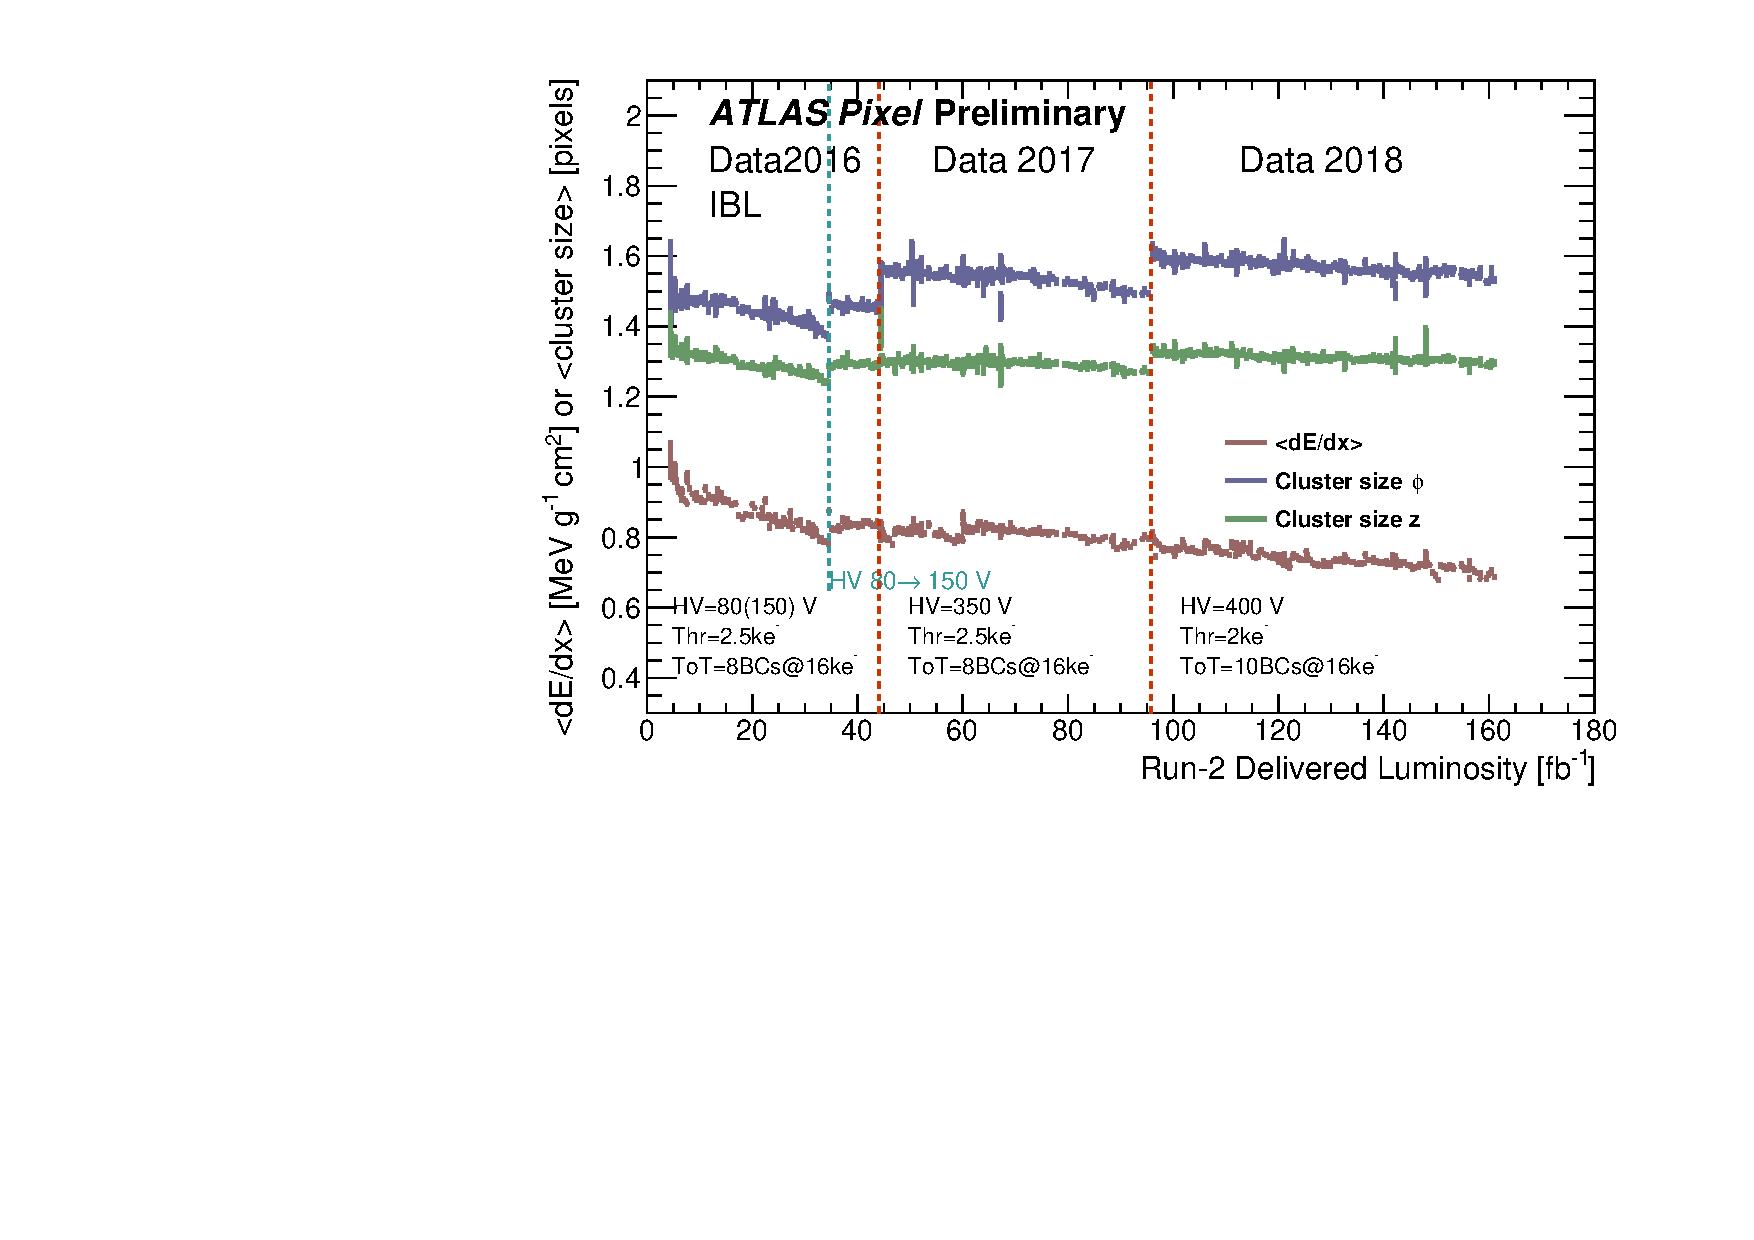
\includegraphics[width=0.8\textwidth]{figures/SensorMeasurements/ChargeCollection/fig_02.pdf}
\caption{Figure from Ref.~\cite{ATL-PIX-2018-011}.}
\label{lab:sensormeasurements:CCE:ATLAS1}
\end{figure}

\subsubsection{Lorentz Angle}

Fig.~\ref{lab:sensormeasurements:Lorentz:ATLAS1}.

\begin{figure}[h!]
\centering
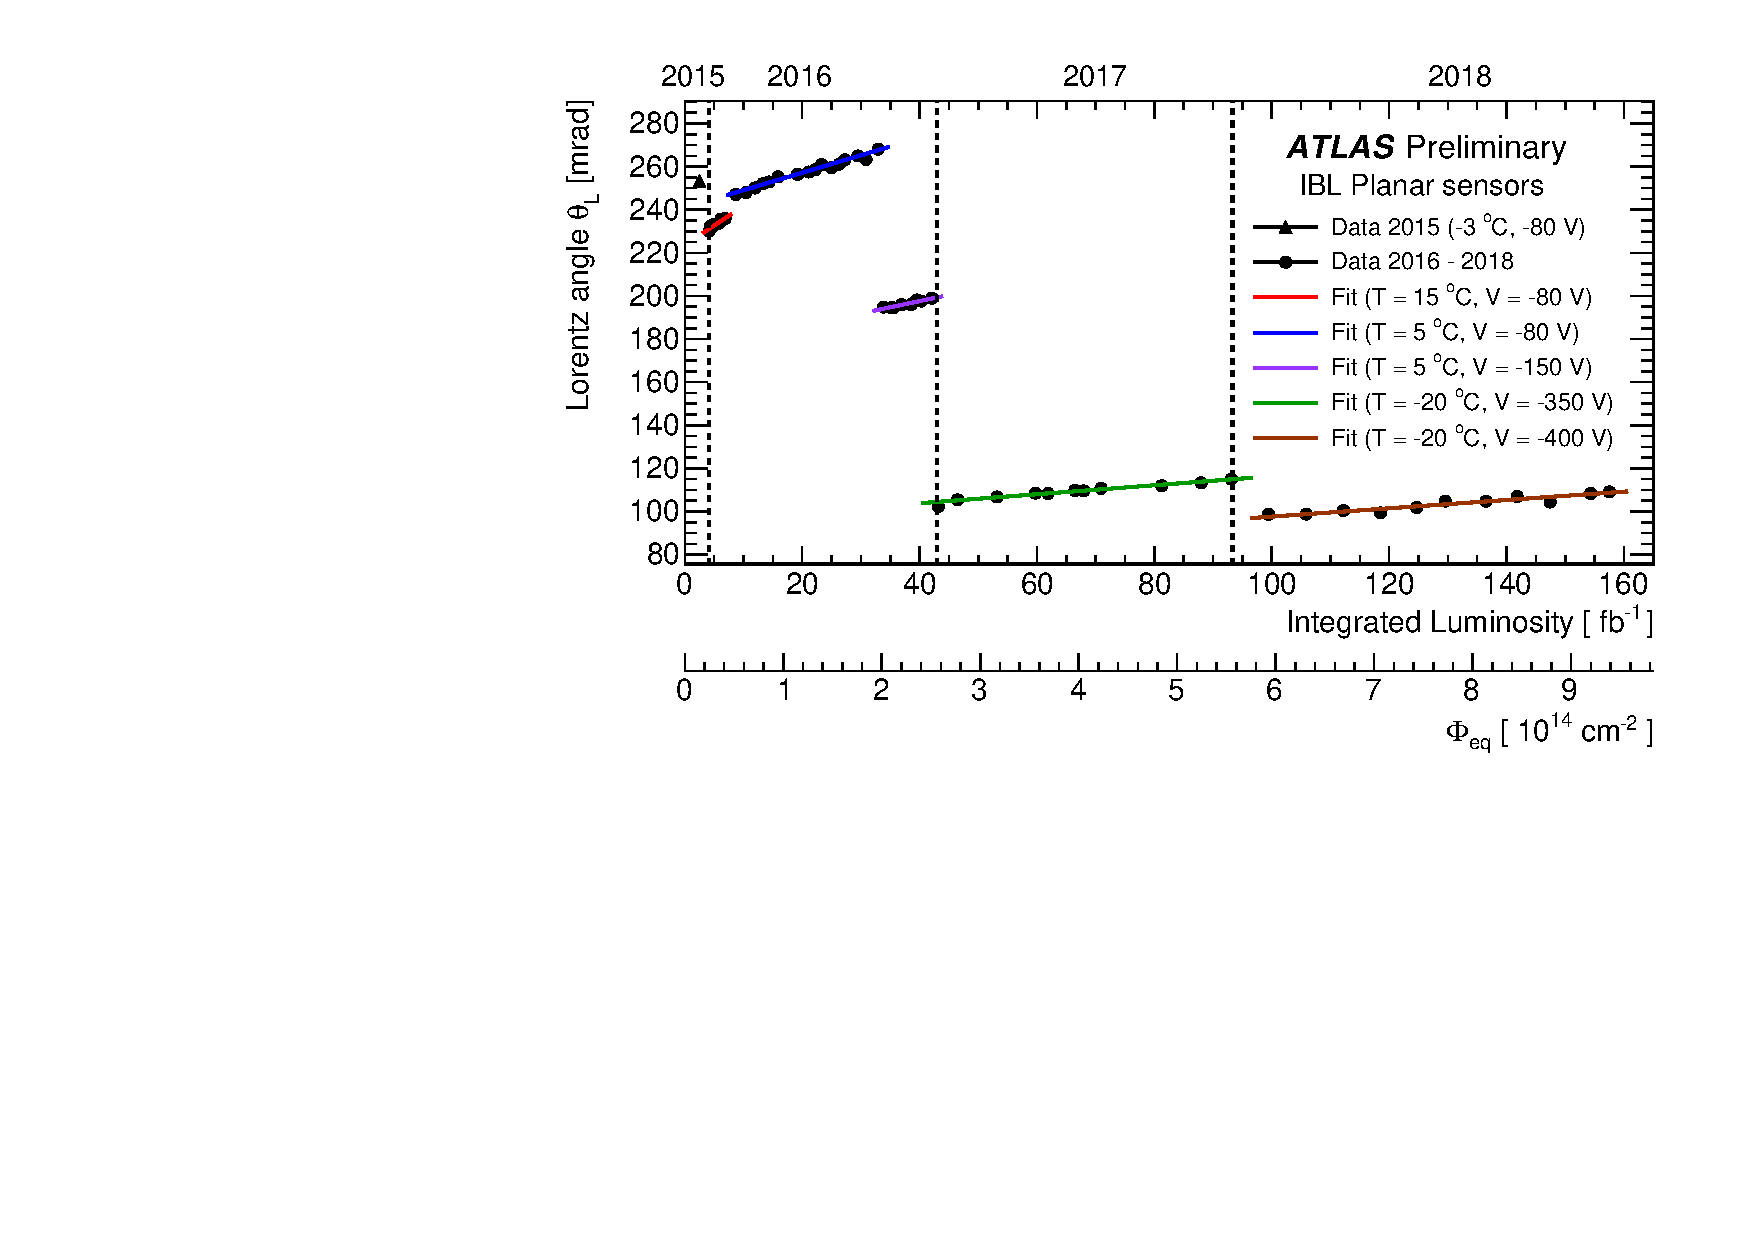
\includegraphics[width=0.8\textwidth]{figures/SensorMeasurements/LorentzAngle/fig_13}
\caption{Figure from Ref.~\cite{ATL-PIX-2017-005}.}
\label{lab:sensormeasurements:Lorentz:ATLAS1}
\end{figure}

\subsubsection{Position Resolution}

Fig.~\ref{lab:sensormeasurements:positionresolution:ATLAS}.

\begin{figure}[h!]
\centering
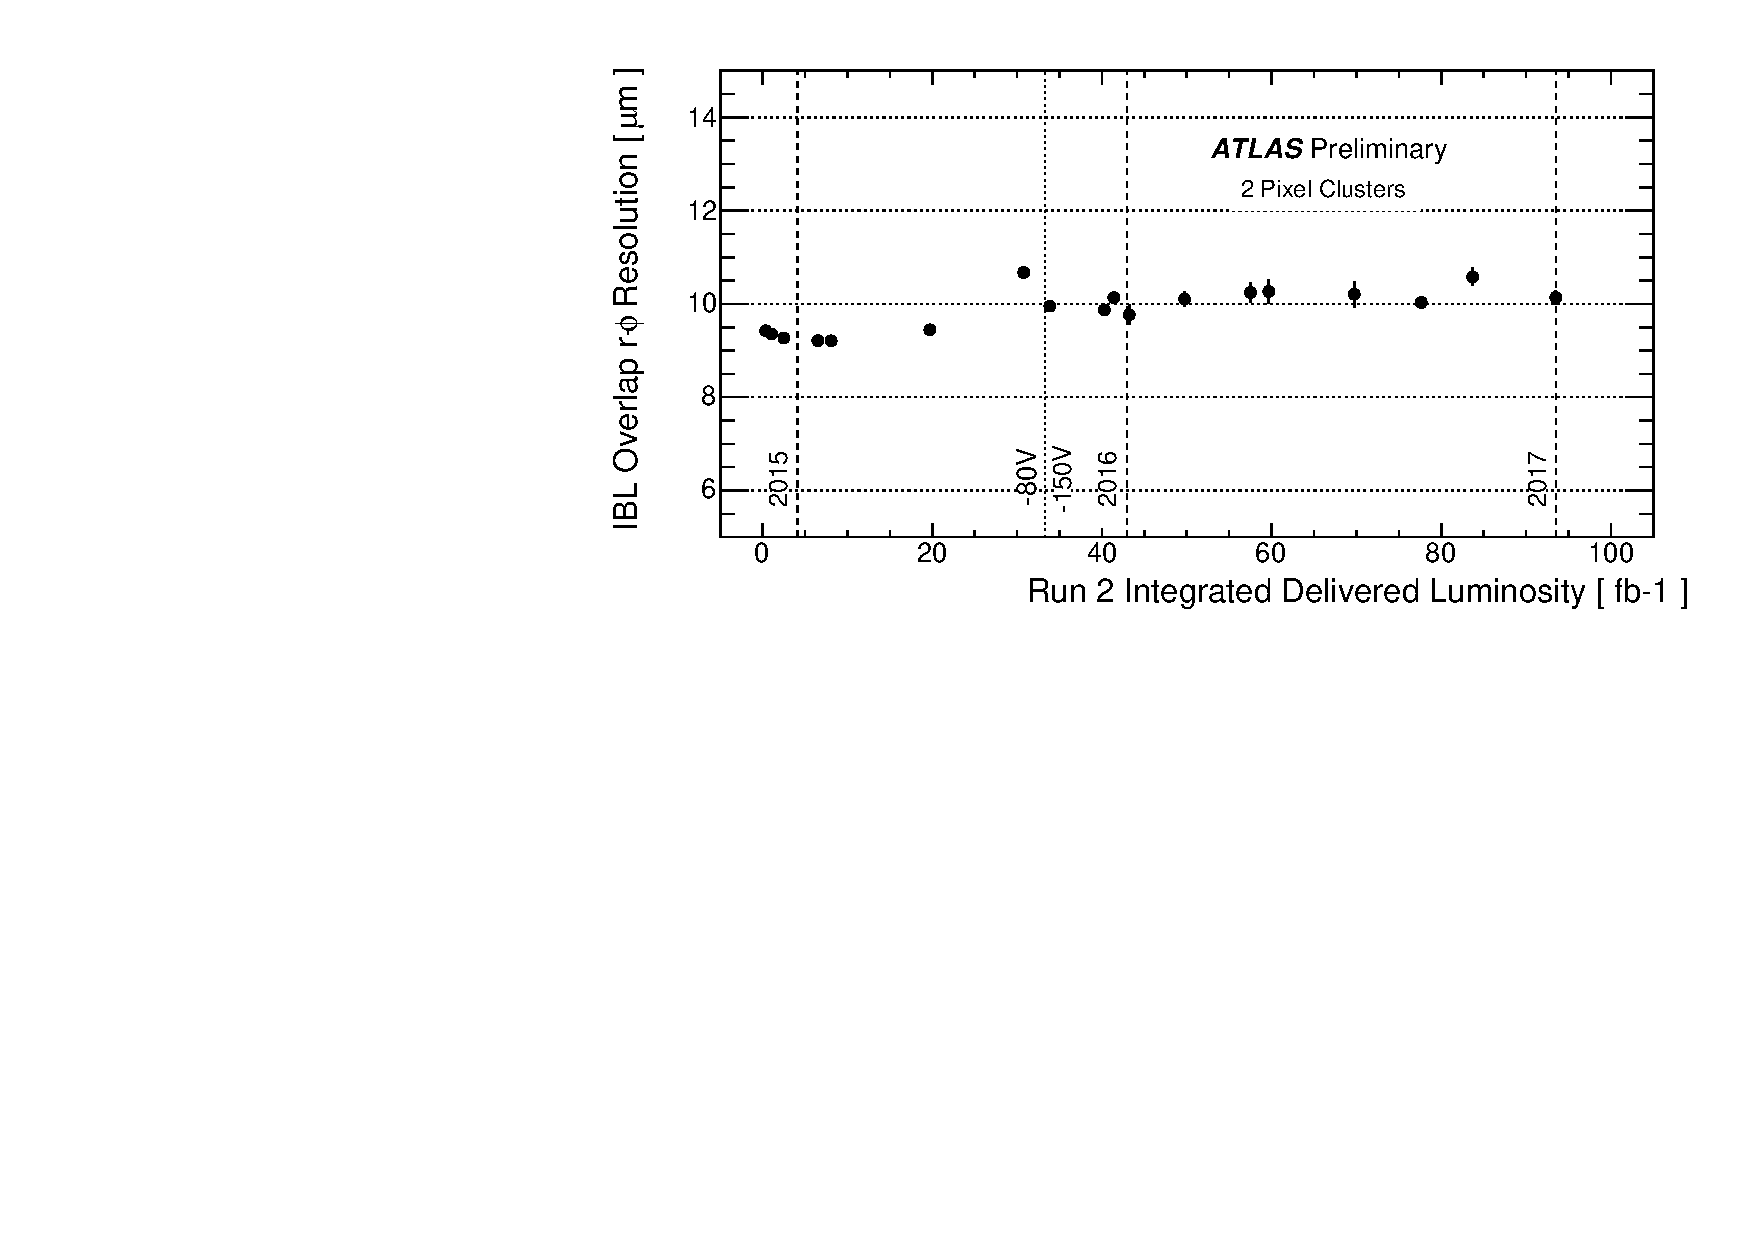
\includegraphics[width=0.8\textwidth]{figures/SensorMeasurements/PositionResolution/fig_01.pdf}
\caption{Figure from Ref.~\cite{ATL-PIX-2018-002}.}
\label{lab:sensormeasurements:positionresolution:ATLAS}
\end{figure}

\subsection{Inter-experiment comparisons}

\subsubsection{Model Parameters}

The idea of this section is to compare Hamburg model parameters.

\subsubsection{Measured Fluence}

Fig.~\ref{lab:sensormeasurements:blah}.

\begin{figure}[h!]
\centering
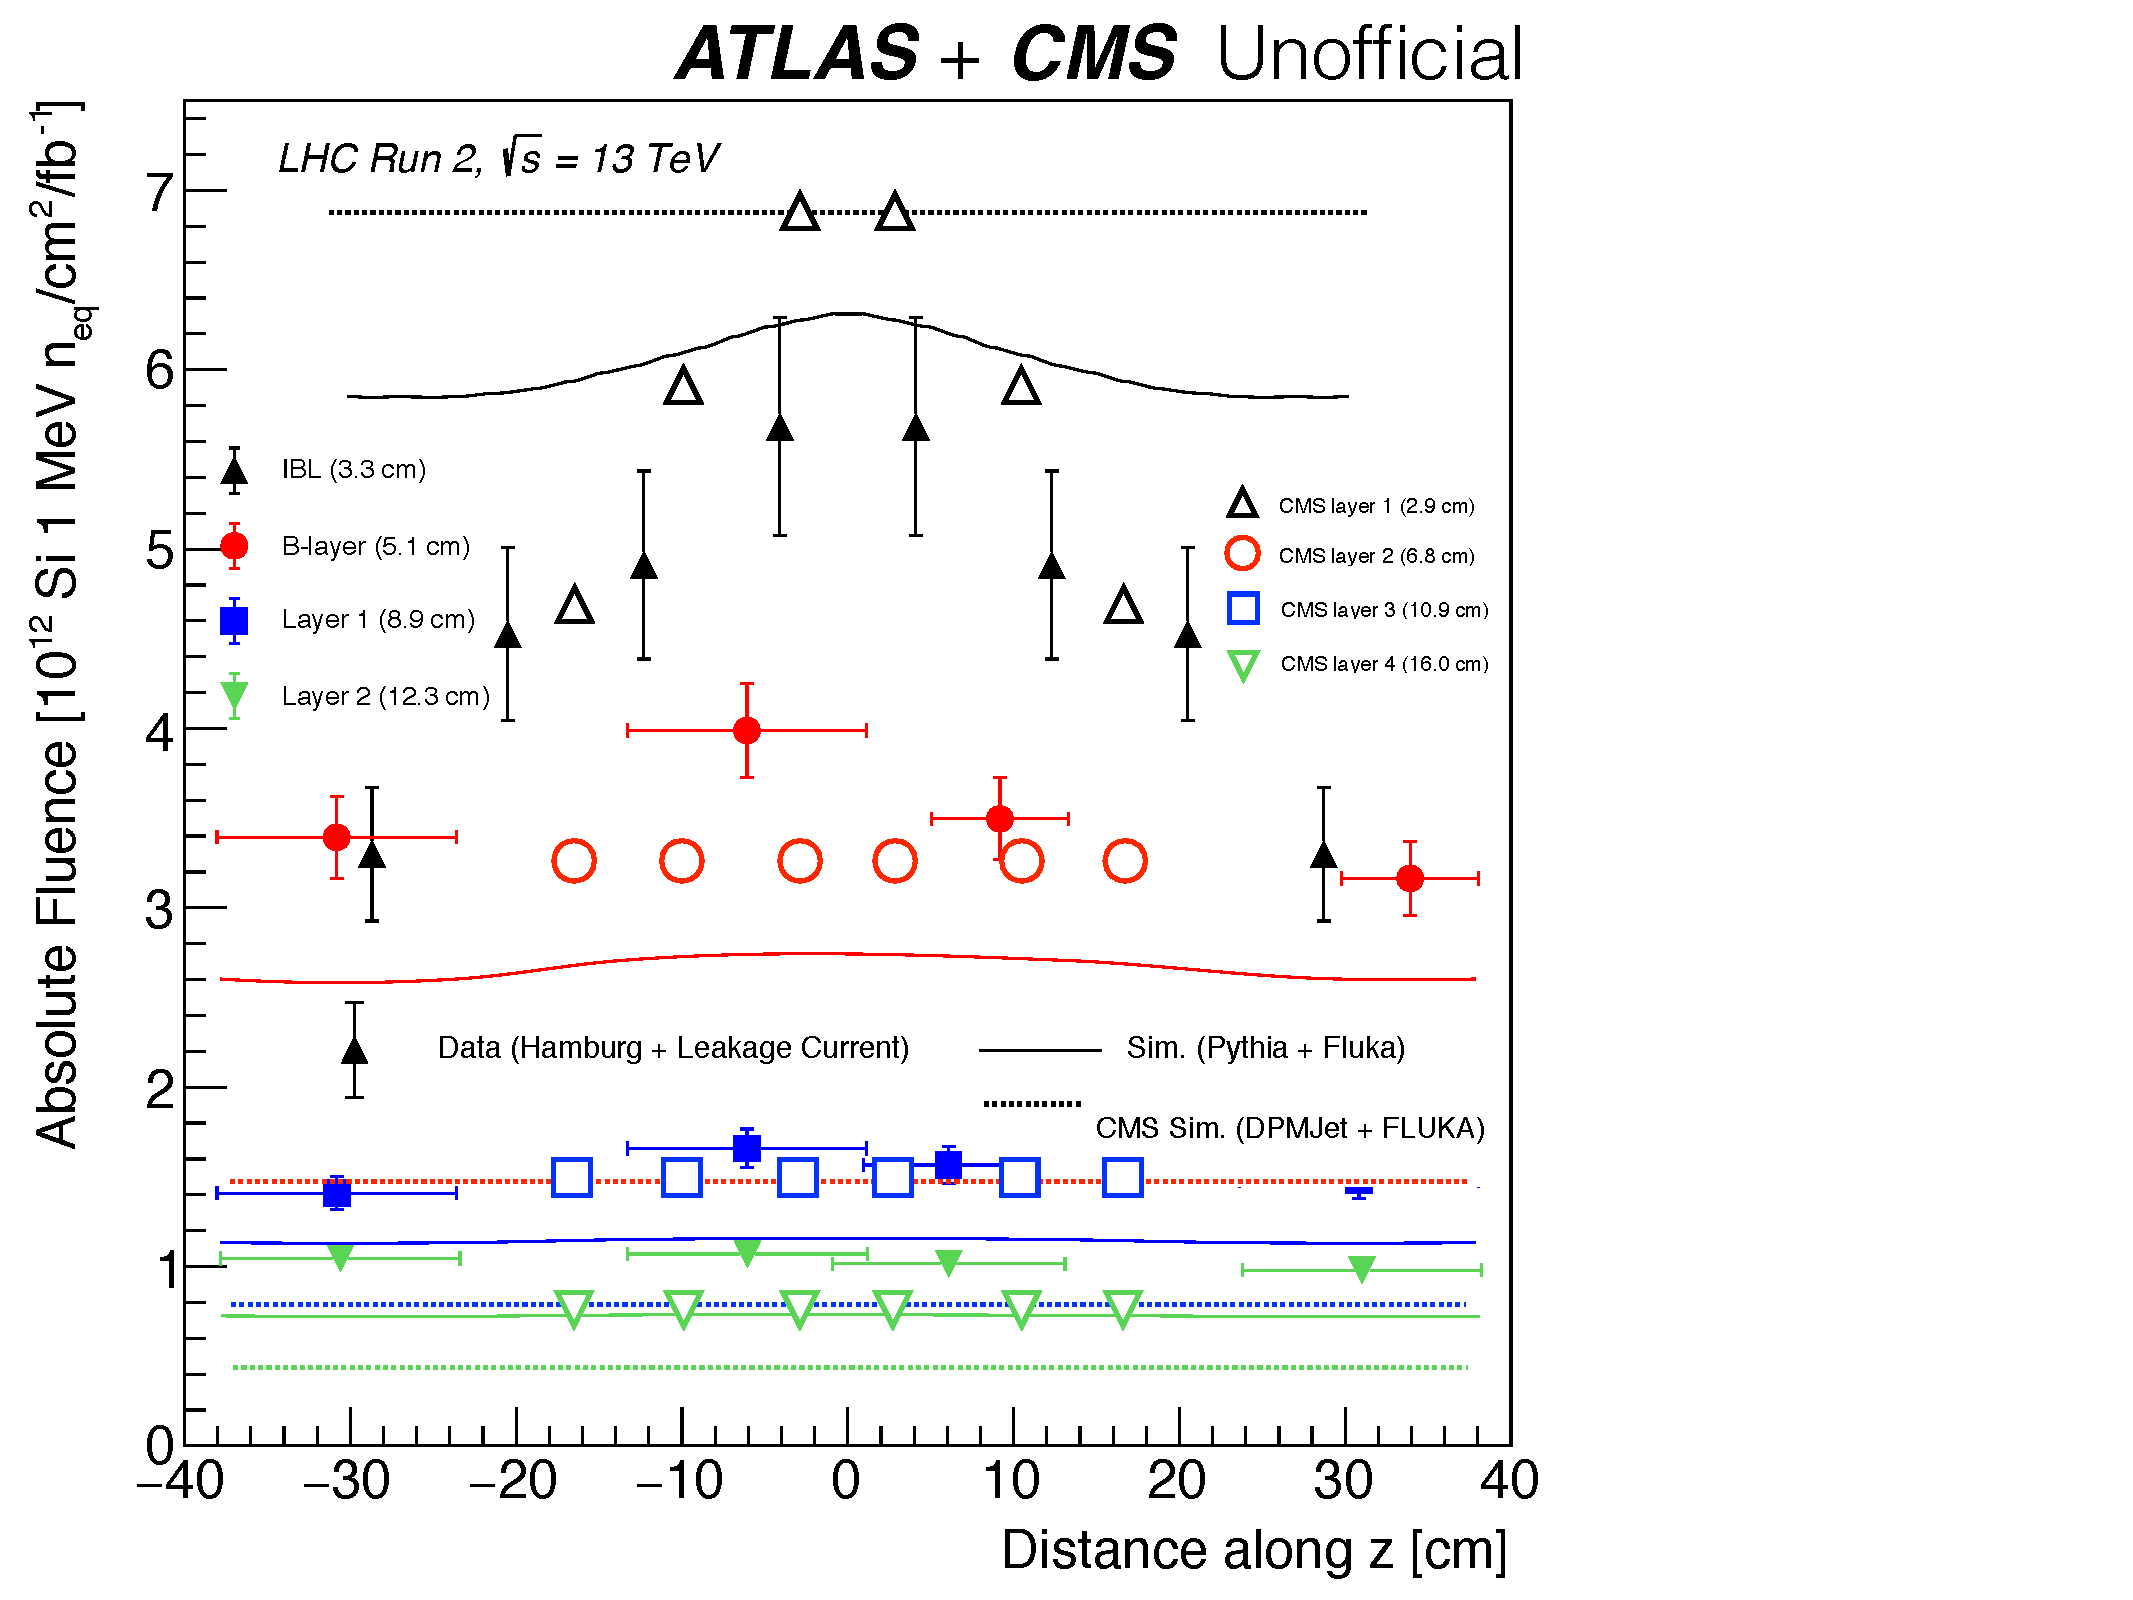
\includegraphics[width=0.5\textwidth]{figures/SensorMeasurements/CombinationPlot}
\caption{blah}
\label{lab:sensormeasurements:blah}
\end{figure}

%\subsection{Extracting fluence from measurements}

\subsection{Discussion}
Drawing conclusions from across the experiments. 
 
\begin{thebibliography}{99}
\end{thebibliography}
